
\documentclass{beamer} 


\mode<presentation>
{
  \usetheme{Berkeley}
  % or ...

  \setbeamercovered{transparent}
  % or whatever (possibly just delete it)
}

\usepackage{tikz}
\usepackage{graphicx}
\usepackage[english]{babel}
% or whatever

\usepackage[utf8]{inputenc}
% or whatever

\usepackage{times}
\usepackage[T1]{fontenc}
% Or whatever. Note that the encoding and the font should match. If T1
% does not look nice, try deleting the line with the fontenc.


\title[] % (optional, use only with long paper titles)
{The Frontier of Research Transparency in the Social Sciences}

\subtitle
{}

\author[Christensen] % (optional, use only with lots of authors)
{Garret~Christensen\inst{1}}
% - Give the names in the same order as the appear in the paper.
% - Use the \inst{?} command only if the authors have different
%   affiliation.

\institute[Universities of Somewhere and Elsewhere] % (optional, but mostly needed)
{
  \inst{1}%
  UC Berkeley:\\
  Berkeley Initiative for Transparency in the Social Sciences\\
  Berkeley Institute for Data Science\\
  }
% - Use the \inst command only if there are several affiliations.
% - Keep it simple, no one is interested in your street address.

\date[BITSS2016] % (optional, should be abbreviation of conference name)
{BITSS 2016 Summer Institute\\
Slides available online at \url{http://www.github.com/BITSS/SummerInstitute2016}}
% - Either use conference name or its abbreviation.
% - Not really informative to the audience, more for people (including
%   yourself) who are reading the slides online

\subject{Research Transparency}
% This is only inserted into the PDF information catalog. Can be left
% out. 

\pgfdeclareimage[height=2cm]{university-logo}{../Images/BITSSlogo.png}
\logo{\pgfuseimage{university-logo}}

% If you have a file called "university-logo-filename.xxx", where xxx
% is a graphic format that can be processed by latex or pdflatex,
% resp., then you can add a logo as follows:

% \pgfdeclareimage[height=0.5cm]{university-logo}{university-logo-filename}
% \logo{\pgfuseimage{university-logo}}



% Delete this, if you do not want the table of contents to pop up at
% the beginning of each subsection:
%\AtBeginSubsection[]
%{
%  \begin{frame}<beamer>{Outline}
%    \tableofcontents[currentsection,currentsubsection]
%  \end{frame}
%}


% If you wish to uncover everything in a step-wise fashion, uncomment
% the following command: 

\beamerdefaultoverlayspecification{<+->}


\begin{document}

\begin{frame}
  \titlepage
\end{frame}




% Structuring a talk is a difficult task and the following structure
% may not be suitable. Here are some rules that apply for this
% solution: 

% - Exactly two or three sections (other than the summary).
% - At *most* three subsections per section.
% - Talk about 30s to 2min per frame. So there should be between about
%   15 and 30 frames, all told.

% - A conference audience is likely to know very little of what you
%   are going to talk about. So *simplify*!
% - In a 20min talk, getting the main ideas across is hard
%   enough. Leave out details, even if it means being less precise than
%   you think necessary.
% - If you omit details that are vital to the proof/implementation,
%   just say so once. Everybody will be happy with that.
%%%%%%%%%%%%%%%%%%%%%%%%%%%%%%%%%%%%%%%%%%%%%%%%%%%%%%%%%%%%%%%%%%%%%%%
%%%%%%%%%%%%%%%%%%%%%%%%%%%%%%%%%%%%%%%%%%%%%%%%%%%%%%%%%%%%%%%%%%%%%

\section {Introduction}
{ % all template changes are local to this group.
    \setbeamertemplate{navigation symbols}{}
    \begin{frame}[plain]
        \begin{tikzpicture}[remember picture,overlay]
            \node[at=(current page.center)] {
                \href{https://www.bitss.org/}{\includegraphics[width=\paperwidth]{../Images/bitsslogo.png}}
            };
        \end{tikzpicture}
     \end{frame}
}

%%%%%%%%%%%%%%%%%%%%%%%%%%%%%%%%%%%%%%%%%%%%%%%%%%%%%%%%%%%%%%%%%%%%%%%%
%%%%%%%%%%%%%%%%%%%%%%%%%%%%%%%%%%%%%%%%%%%%%%%%%%%%%%%%%%%%%%%%%%
\section{Study Design and Power}
\begin{frame}{Study Design and Power}
Practical suggestion to adequately power trials to help prevent spurious significant results.
\begin{itemize}
\item
Collaborate with other labs to mutually run each others' experiments (Open Science Collaboration 2014, 2015).
\begin{itemize}[<.->]
\item \href{http://science.sciencemag.org/content/349/6251/aac4716.full}{Replication Project: Psychology}
\item \href{http://econtent.hogrefe.com/doi/full/10.1027/1864-9335/a000178}{Many Labs 1}, \href{https://osf.io/8cd4r/}{2}, 3
\item Crowdsourcing Analysis \href{http://www.nature.com/news/crowdsourced-research-many-hands-make-tight-work-1.18508}{(Silberzahn and Uhlmann 2016)}
\item \href{http://science.sciencemag.org/content/early/2016/03/02/science.aaf0918}{Experimental economics replications (Camerer et al. 2016)}
\end{itemize}
\end{itemize}

\end{frame}

{ % all template changes are local to this group.
    \setbeamertemplate{navigation symbols}{}
    \begin{frame}[plain]
        \begin{tikzpicture}[remember picture,overlay]
            \node[at=(current page.center)] {
                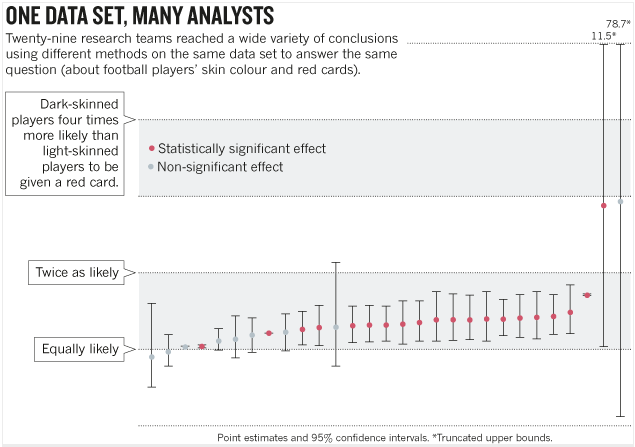
\includegraphics[width=\paperwidth]{../Images/Crowdsourcing2.PNG}
            };
        \end{tikzpicture}
     \end{frame}
}
%%%%%%%%%%%%%%%%%%%%%%%%%%%%%%%%%%%%%%%%%%%%%%%%%%%%%%%%%%%%%%%%%%%%%
\section{Registrations}


\begin{frame}{Registration}
\begin{itemize}
   \item Newer to social sciences, but:
   \begin{itemize}[<.->]
   \item
   	AEA registry, currently only for RCTs. \url{http://socialscienceregistry.org}
   \item
    EGAP registry \url{http://egap.org/design-registration}
   \item 
    3ie registry, for developing country evaluations. \url{http://ridie.3ieimpact.org}
   \item
   	Open Science Framework\\ \url{http://osf.io}
   	\begin{itemize}
   	\item
   	Open format
   	\item
   	Will soon sync with above
   	\end{itemize}
   \end{itemize}
  \end{itemize}  
\end{frame}

 { % all template changes are local to this group.
    \setbeamertemplate{navigation symbols}{}
    \begin{frame}[plain, label=AEAreg]
         \begin{tikzpicture}[remember picture,overlay]
            \node[at=(current page.center)] {
                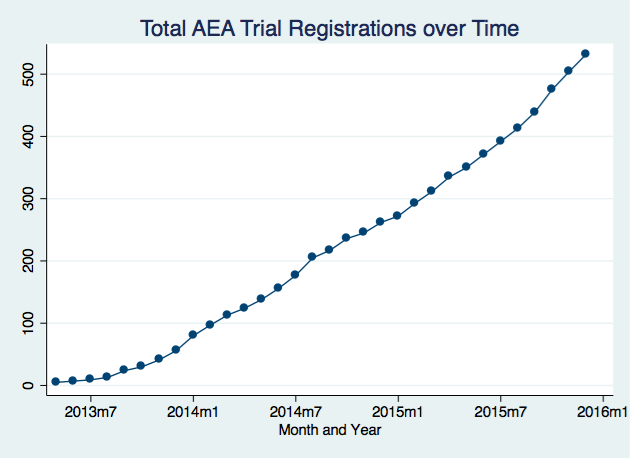
\includegraphics[height=\paperheight]{../Images/AEARegistrations.PNG}
            };
        \end{tikzpicture}
     \end{frame}
}

{ % all template changes are local to this group.
    \setbeamertemplate{navigation symbols}{}
    \begin{frame}[plain, label=AEAreg]
         \begin{tikzpicture}[remember picture,overlay]
            \node[at=(current page.center)] {
                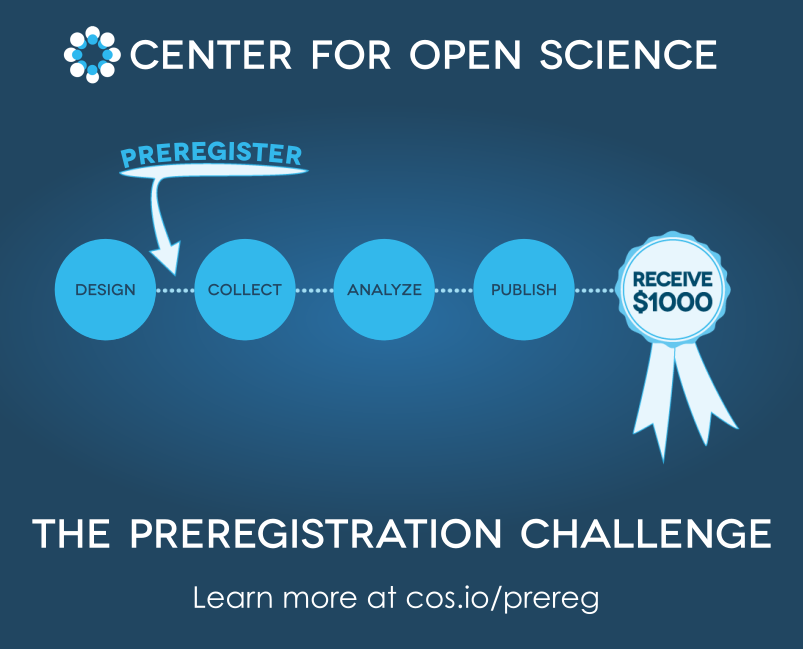
\includegraphics[width=\paperwidth]{../Images/preregchallenge.png}
            };
        \end{tikzpicture}
     \end{frame}
}


\begin{frame}{Design-Based Publication}
AKA Registered Reports, moves peer review before data gathering, results, and analysis.

\begin{enumerate}[<.->]
\item Design a project
\item Submit
\item Reviewed based on importance of question and quality of design
\item Get in-principle acceptance
\item Follow through, and nulls get published
\end{enumerate}
\href{https://osf.io/8mpji/wiki/home/}{20 Journals, 5 more with Special Issues \beamergotobutton{Link}}
\end{frame}

{ % all template changes are local to this group.
    \setbeamertemplate{navigation symbols}{}
    \begin{frame}[plain, label=AEAreg]
         \begin{tikzpicture}[remember picture,overlay]
            \node[at=(current page.center)] {
                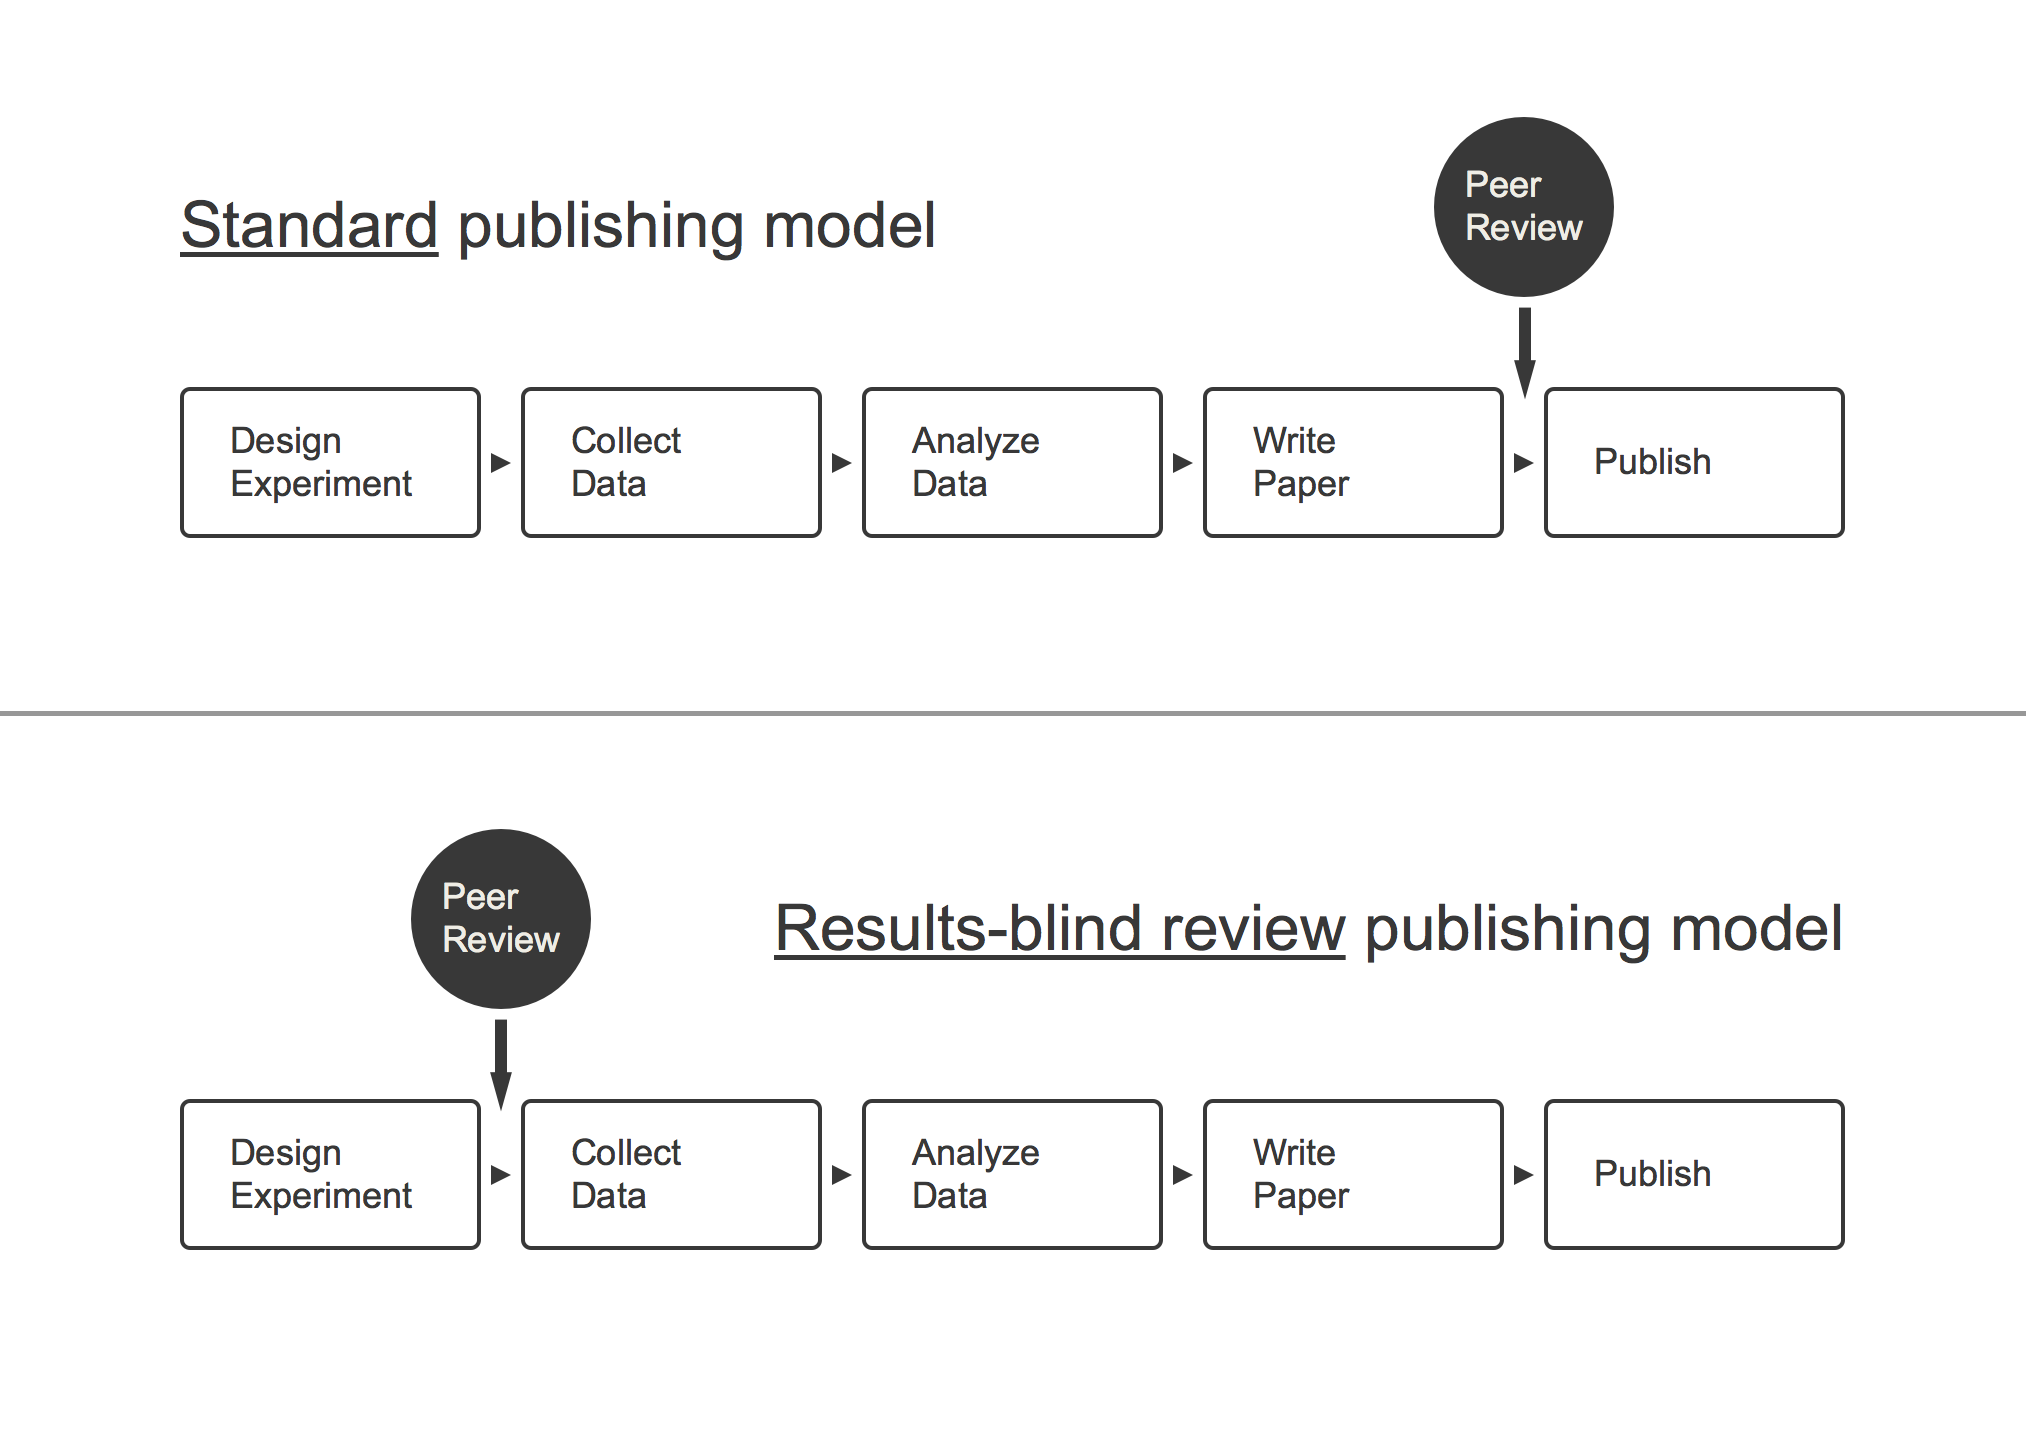
\includegraphics[height=\paperheight]{../Images/results_blind_review.png}
            };
        \end{tikzpicture}
     \end{frame}
}



\subsection*{Project Protocol, Reporting Standards}
\begin{frame}[<.->]{Project Protocol, Reporting Standards}
 Make sure you report everything another researcher would need to replicate your research.
 \begin{itemize}
 \item Find the appropriate reporting standard for your field and follow it: \url{http://www.equator-network.org}
\item Report the nuts and bolts of the project implementation in a detailed protocol: \url{http://www.spirit-statement.org}
\item Transparency and Openness Promotion (TOP) Guidelines: \url{http://cos.io/top}
\end{itemize}
\end{frame}

 { % all template changes are local to this group.
    \setbeamertemplate{navigation symbols}{}
    \begin{frame}[plain, label=AEAreg]
         \begin{tikzpicture}[remember picture,overlay]
            \node[at=(current page.center)] {
                
\includegraphics[width=\paperwidth]{../Images/TOPGuidelines.PNG}
            };
        \end{tikzpicture}
     \end{frame}

 \setbeamertemplate{navigation symbols}{}
    \begin{frame}[plain, label=AEAreg]
         \begin{tikzpicture}[remember picture,overlay]
            \node[at=(current page.center)] {
                
\includegraphics[width=\paperwidth]{../Images/TakingUpTop.PNG}
            };
        \end{tikzpicture}
     \end{frame}
    }



\subsection*{Data Sharing}
\begin{frame}{Data Sharing}
Post your code and your data in a trusted public repository.
\begin{itemize}[<.->]
\item
Find the appropriate repository: \url{http://www.re3data.org/}
\item
Repositories will last longer than your own website.
\item
Repositories are more easily searchable by other researchers.
\item
Repositories will store your data in a non-proprietary format that won't become obsolete.
\end{itemize}
\end{frame}

\begin{frame}{``Stupid Little Badges''}
\href{https://cos.io/pr/2016-05-12/}{Publish in a journal that `rewards' good behavior.}

538: ``Even pyschologists respond to meaningless rewards''

\vspace{0.5in}

\includegraphics[scale=0.5]{../Images/materials.png}

\includegraphics[scale=0.5]{../Images/preregistered.png}

\includegraphics[scale=0.5]{../Images/data.png}

\end{frame}

{
 \setbeamertemplate{navigation symbols}{}
    \begin{frame}[plain, label=AEAreg]
         \begin{tikzpicture}[remember picture,overlay]
            \node[at=(current page.center)] {
                \includegraphics[height=\paperheight]{../Images/538badges.PNG}
            };
        \end{tikzpicture}
     \end{frame}
    }
{
 \setbeamertemplate{navigation symbols}{}
    \begin{frame}[plain, label=AEAreg]
         \begin{tikzpicture}[remember picture,overlay]
            \node[at=(current page.center)] {
                \includegraphics[width=\paperwidth]{../Images/PRO.PNG}
            };
        \end{tikzpicture}
     \end{frame}
    }



\section{Conclusion}
\begin{frame}{Conclusion}
OK, I'm convinced. How do I implement this in my own research?

\begin{itemize}[<.->]
\item Read the manual I wrote.\href{https://github.com/garretchristensen/BestPracticesManual}{\beamergotobutton{Link}}
\item Subscribe to the BITSS blog \& E-mail list \href{https://bitss.org/blog}{\beamergotobutton{Link}}
\item Apply for our Summer Institute. \href{http://www.bitss.org/events/summer-institute/}{\beamergotobutton{Link}}
\item Apply for our SSMART Grants (extra funding for developing country researchers). \href{http://www.bitss.org/ssmart-grants/}{\beamergotobutton{Link}}

\item Apply for our Leamer-Rosenthal Prizes. \href{http://www.bitss.org/lr-prizes/}{\beamergotobutton{Link}}
\end{itemize}
\end{frame}

\begin{frame}{Summer Institute}
Here at UC Berkeley, in July at the University of Michigan, good chance of abroad next year.
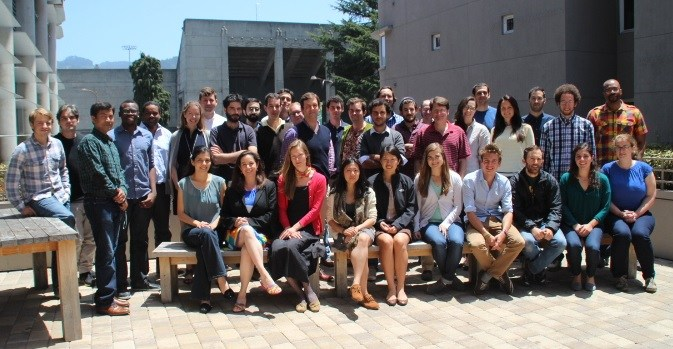
\includegraphics[width=4in]{../Images/bitss-2014-cohort2.jpg}
\end{frame}

\begin{frame}{SSMART Grant}
Up to \$30,000 grant for a research project on:
\begin{itemize}[<.->]
\item Develop new methodology
\item New tools and approaches for meta-analysis
\item Research on researchers and adoption of new norms
\end{itemize}
Extra funding source for researchers from developing countries.

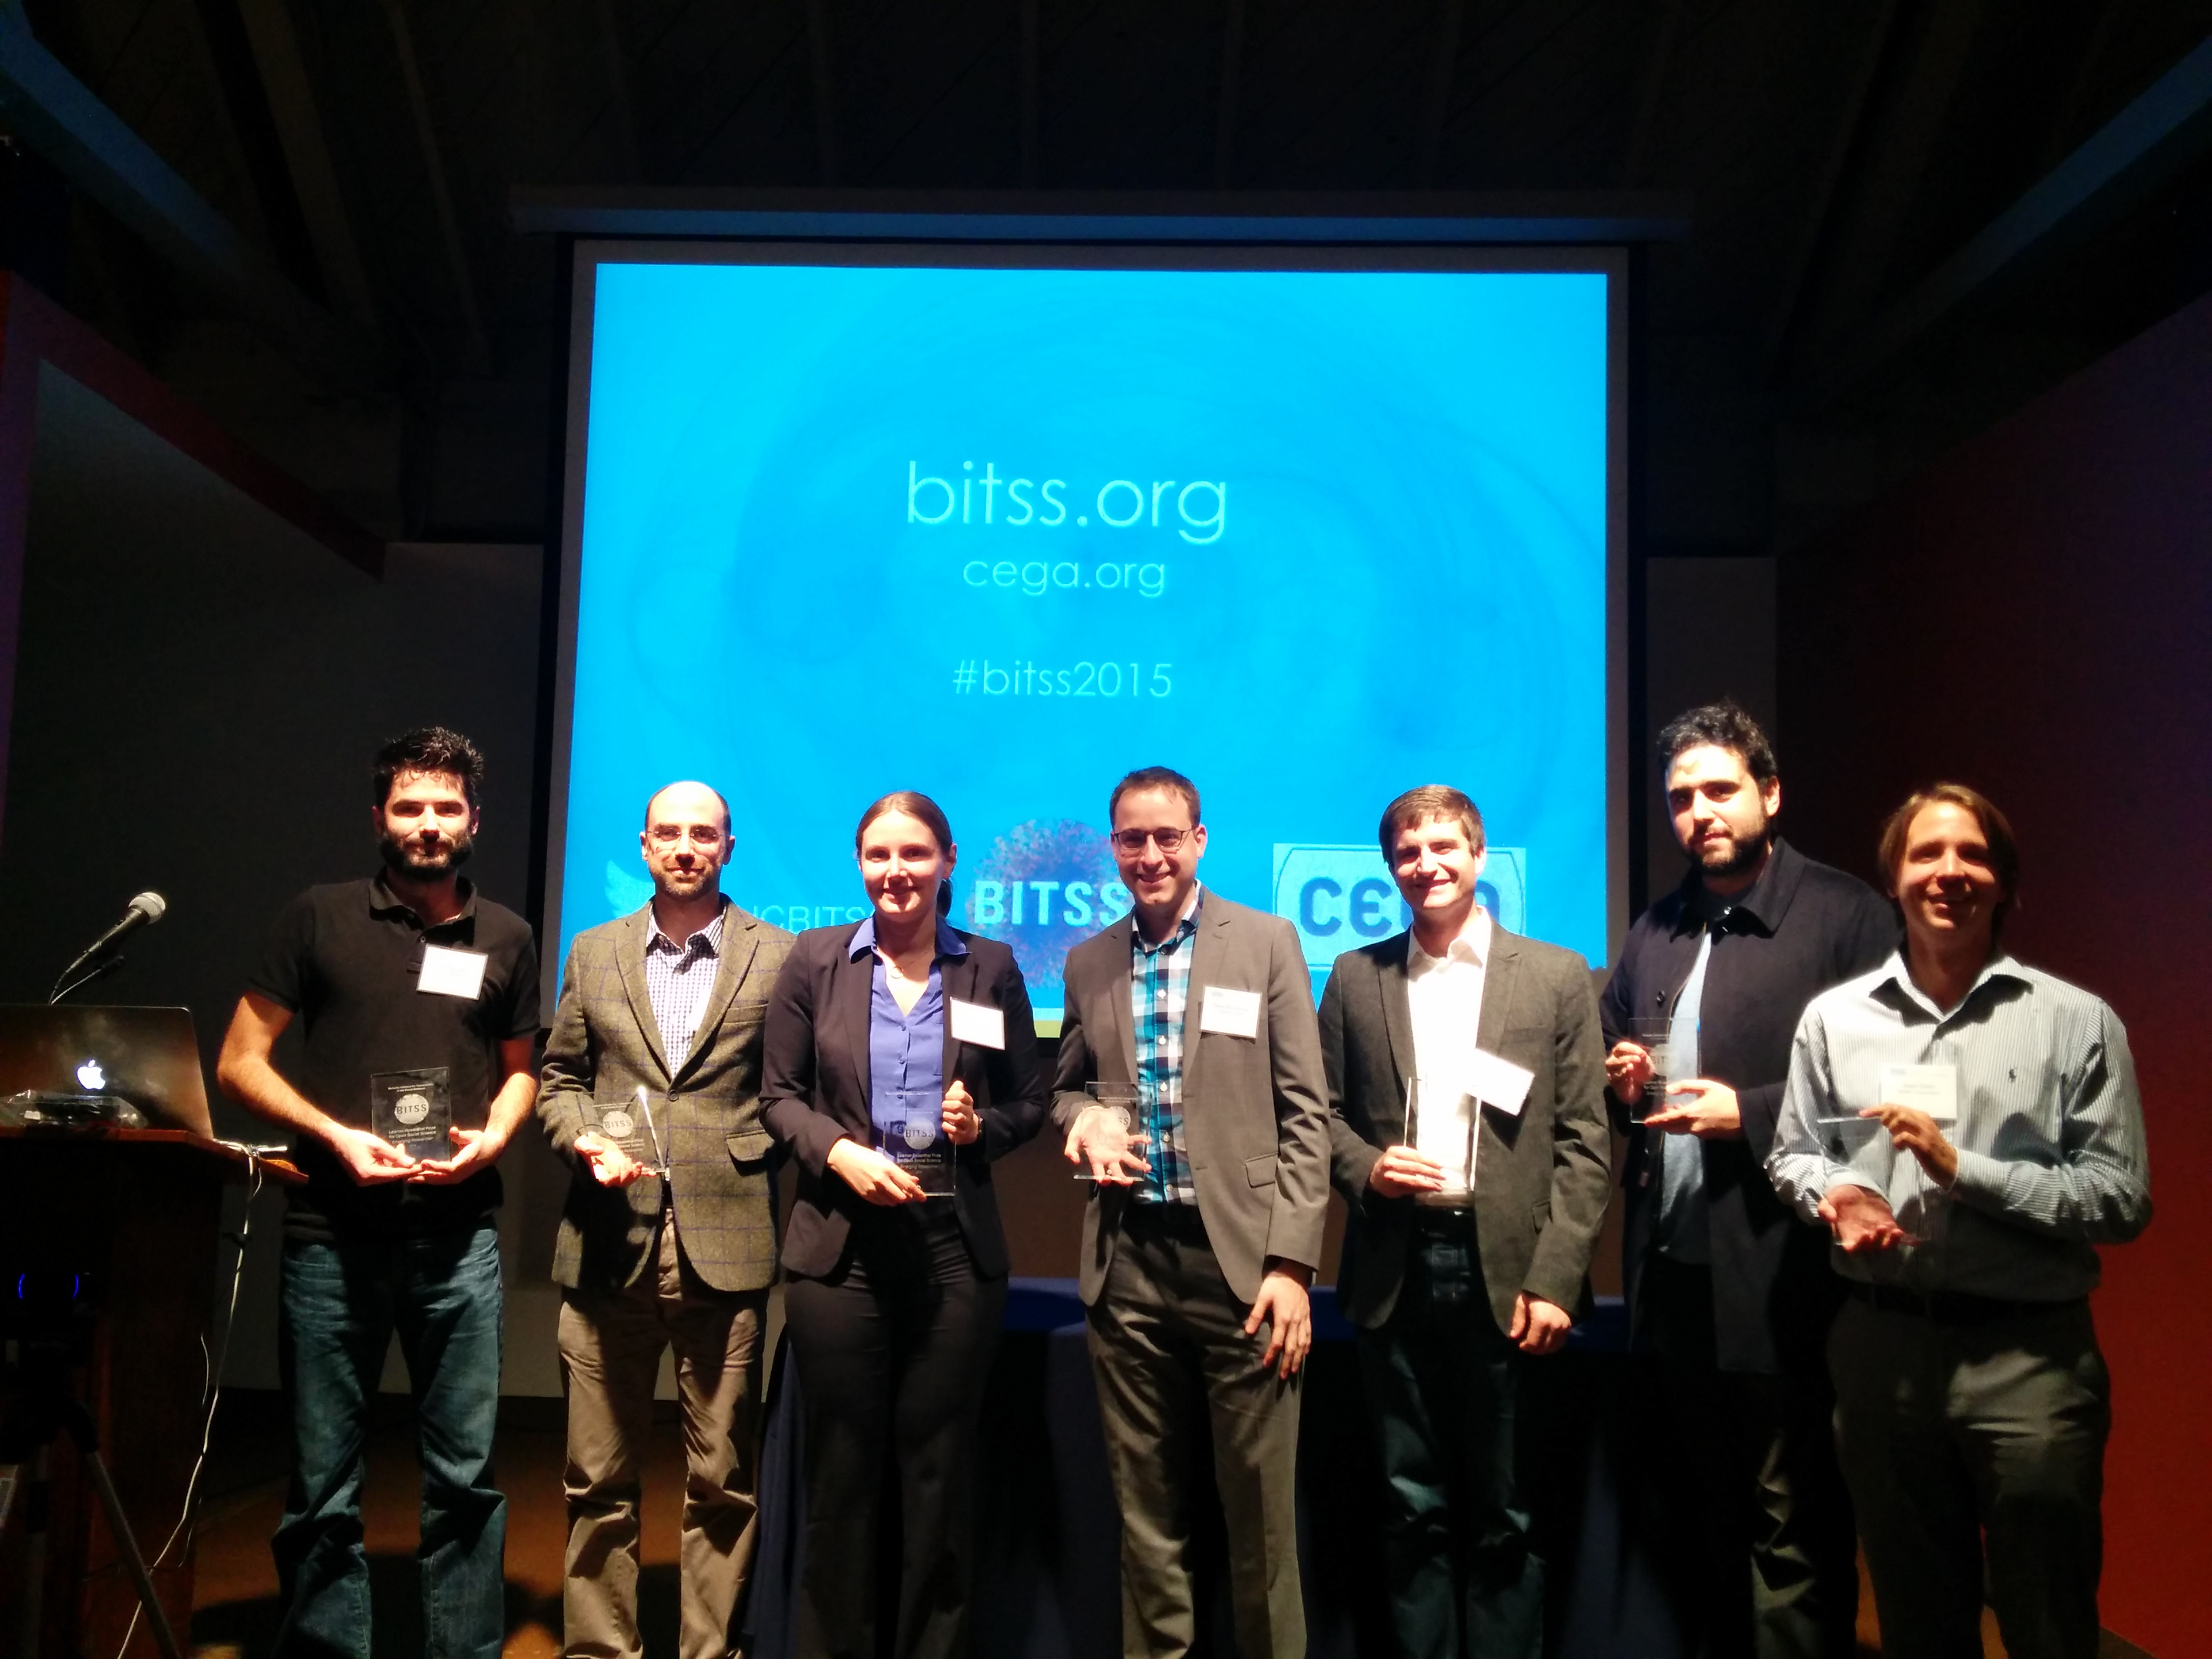
\includegraphics[width=2.5in]{../Images/LRwinners.jpg}
\end{frame}

\begin{frame}{Leamer-Rosenthal Prizes}
Up to \$10,000 prize for completed transparent research in the social sciences,
especially:
\begin{itemize}[<.->]
\item Economics
\item Political Science
\item Psychology
\end{itemize}
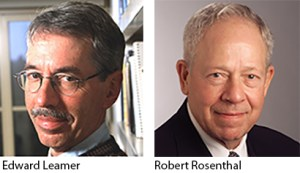
\includegraphics[width=2.5in]{../Images/leamer1-zoomed33.jpg}
\end{frame}


\begin{frame}{Stay Involved}
Join our \href{http://www.bitss.org/catalysts/}{catalyst network}!
\end{frame}

\begin{frame}
\begin{center}
Questions?
\vspace{1in}


\Huge{Thank you!}
\end{center}
\end{frame}

\end{document}

